% !TeX encoding = UTF-8
% !TeX spellcheck = pt_BR

\chapter{Proposta de atividade e \textit{Hands on!}}
\chaptermark{Atividade e \textit{Hands on!}}

\begin{flushright}
	\begin{minipage}{8cm}
		\textit{	\noindent 
			\begin{flushright}
				``Montamos uma pequena operação de mineração de bitcoin e ethereum... que milagrosamente agora está ganhando muito dinheiro'' - Abigail Johnson (tradução livre)
		\end{flushright}}
		\vspace{1cm} 
	\end{minipage}
	\footnote{Citação original do inglês: ``We set up a small bitcoin and ethereum mining operation…that miraculously now is actually making a lot of money.'' em reportagem \cite{TECHCRUNCH}}.
\end{flushright}

Neste capítulo é exibida uma atividade desenvolvida pelo autor do presente instrumento que mostra aos alunos o custos e ganhos na mineração de criptomoedas, além do cálculo do tempo de retorno do investimento de um hardware apropriado.

\section{Introdução} \index{Interdisciplinaridade}
Neste capítulo, uma simples proposta de atividade será apresentada. Esta atividade pode ser aplicada com discentes do ensino fundamental e envolve conhecimentos de matemática financeira, conversões de medidas, sobre capacidade computacional de computadores e ainda há a oportunidade da interdisciplinaridade com turmas de história\footnote{Aqui supondo alguma base histórica sobre valores monetários, história da criptografia} ,turmas de geografia \footnote{Conceitos de globalização ou circulação de capital se aplicam bem aqui}, ou até em turmas de língua  inglesa ou língua espanhola\footnote{Aqui podemos explorar que a mineração pode ocorrer em qualquer lugar do mundo, estudar sobre como a leitura de website em língua inglesa ou espanhola podem abrir novos possibilidades para os alunos}. 

A ideia da atividade é introduzir ao aluno sobre a existência de algoritmos de mineração já bastante difundido pela comunidade de mineração,\index{Mineração} como por exemplo \textit{Ethash}, \index{Ethereum} \textit{Ethash4G}, \textit{KawPow} e \textit{MTP} e juntamente com a calculadora de lucros \textit{Whattomine} \index{Whattomine} \footnote{Você pode aprender mais sobre esta ferramenta acesso seu endereço em \cite{WTM}} obter alguns cálculos convertendo gasto energético em lucro. Por último, gostariamos de estimar o tempo estimado da recuperação dos investimentos em hardware, \index{Hardware} novamente segundo os cálculos da calculadora de lucros e uma tabela de cálculo desenvolvida pelo autor deste presente instrumento.\\

\subsection{Motivador para a atividade}
Você leitor, tem interesse em minerar criptomoedas e não sabe calcular se essa atividade "vale a pena"? Com as altas taxas de desemprego atualmente em nosso país, muitas pessoas hoje em dia já estão fazendo rendas extras e até como renda principal a mineração de criptomoedas. Imagine a seguinte situação: Um motorista por aplicativo para adquirir um veículo novo deve investir uma média de 20 a 30 mil reais. Supondo que este motorista tenha uma certa renda bruta, excluiria-se daí então uma grande porção em combustível, taxas veículares, multas e manutenções, excluindo ainda o fator segurança. Em quanto tempo este motorista recuperaria seu investimento? Ao final deste capítulo, um comparativo será possivel. \label{motiv}      

\begin{figure}[H] \index{Dogecoin} \index{Ethereum} \index{Tesla} \index{Criptomoeda}
	\centering
	\caption{Um passeio veicular com Dogecoin e Ethereum}
	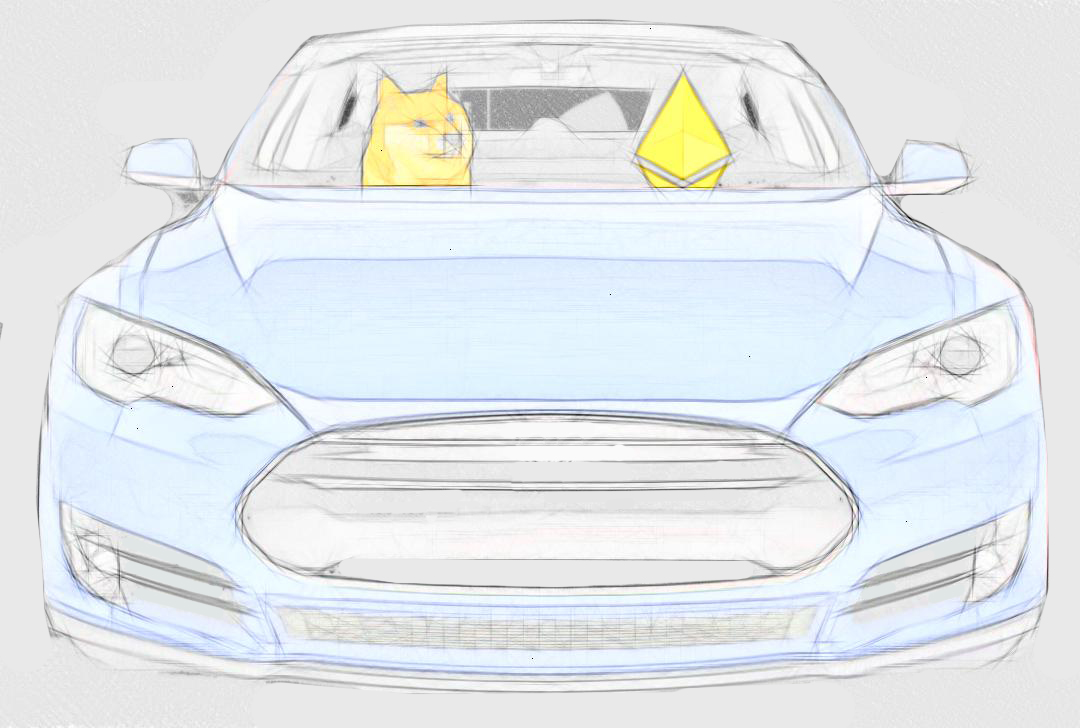
\includegraphics[width=0.7\linewidth]{tesla-ethereum-doge_sketch.jpg}\\
	\text{Fonte: Ilustrado digitalmente pelo autor}
\end{figure}

\section{Embasamento da atividade}
\subsection{Bases necessárias para a atividade}
Conforme relatado no plano de aula do professor, recomenda-se que o conteúdo desta atividade seja inserido num cronograma de aulas de matemática financeira. Conversões de câmbio, conversões de medidas e porcentagens são alguns dos termos que serão usados.

\subsubsection{Matemática Financeira}

A atividade é baseada na importância dos alunos terem um boa literacia, ou letramento financeiro. Segundo \cite{ORTON}, literacia: \index{Literacia}

\begin{citacao}
		Refere-se à capacidade de ler, analisar e interpretar as condições financeiras pessoais que afetam o bem-estar em nível material. Inclui a capacidade de discernir sobre decisões financeiras, discutir sobre dinheiro e assuntos financeiros. Planejar o futuro e responder de forma competente às várias etapas e acontecimentos da vida que afetam as decisões financeiras, incluindo acontecimentos da economia em geral.
	\end{citacao}

 Tal literacia traz um interesse geral tanto para empresas multinacionais tanto para governantes, pois uma nação cuja população possui um ensino rígido em Educação financeira (\textbf{EF}) tem fundamentos para que haja a promoção do crescimento econômico, confiança e estabilidade e complexidade dos mercados financeiros. \index{Educação Financeira} Segundo o \cite{OCDE}, a educação financeira pode ser definida como o processo pelo qual os consumidores/investidores financeiros melhoram sua compreensão de produtos, conceitos e riscos financeiros e através de informações, instruções e/ou conselhos objetivos, desenvolver as habilidades e a confiança para se tornar mais consciente dos riscos e oportunidades financeiras, para fazer escolhas informadas, para saber onde buscar ajuda e tomar outras medidas eficazes para melhorar seu bem-estar financeiro. \\	

Com efeito, tudo começa com o hábito, e para isso, precisamos
ter uma compreensão profunda dos hábitos que podem impactar a capacidade financeira no decorrer da vida e ensinar os alunos ainda pequenos sobre educação financeira faz parte deste processo de crescimento econômico nacional.

\subsubsection{Conversões de medidas} \index{Métricas}
A necessidade de se tomar medidas são muito antiga e se remetem ainda as civilizações primárias. De fato, cada população tinha seu jeito de tomar medidas, onde muita das vezes tais unidades eram imprecisas pois tinham base no corpo humano como pé, polegada, jarda, braça, côvado, palmo, etc. Alguns destes tipos de medição podem ser facilmente encontrados em livros históricos como visto em \cite{CUNHA} e são conhecidos atualmente no sistema imperial\footnote{Alguns destes como  pés, polegadas e jardas são amplamente usado em países como os Estados Unidos da América.}, diferente do sistema internacional de medidas (SI) padronizado que conhecemos\footnote{Leia mais sobre isto em \cite{LEGER}}. Nesta atividade usaremos a escala de armazenamento computacional  e também a escala de hashes, conforme abaixo. 

\begin{table}[H] \label{hashtable}
	\centering
%\begin{tabular}{|c|c|l|}
%	\hline
%	Abreviação  & Leitura & Referência \\
%	\hline
%	1 h/s & 1 hash por segundo &  \\
%	\hline
%	1 KH/s & 1 kilohash por segundo  & 1.000 (mil) de hashes por segundo \\
%	\hline
%	1 MH/s & 1 megahash por segundo & 1.000.000 (um milhão) de hashes por segundo \\
%	\hline
%	1 GH/s & 1 gigahash por segundo & 1.000.000.000 (um bilhão) de hashes por segundo \\
%	\hline
%	1 TH/s & 1 terahash por segundo & 1.000.000.000.000 (um trilhão) de hashes por segundo \\
%	\hline
%	1 PH/s & 1 petahash por segundo & 1.000.000.000.000.000 (um quadrilhão) de hashes por segundo \\
%	\hline
%	1 EH/s & 1 exahash por segundo & 1.000.000.000.000.000.000 (um quinquilhão) de hashes por segundo \\
%	\hline
%\end{tabular}
\index{Métricas}
	\begin{tabular}{|l|p{16mm}|p{16mm}|p{16mm}|p{16mm}|p{16mm}|p{16mm}|p{16mm}|} 
			
		\hline
		&&&&&&&\\
		Abreviação & 1 h/s & 1 KH/s & 1 MH/s & 1 GH/s & 1 TH/s & 1 PH/s & 1 EH/s \\
		&&&&&&&\\
		\hline
		&&&&&&&\\
		Leitura & 1 hash por segundo & 1 kilohash por segundo & 1 megahash por segundo & 1 gigahash por segundo & 1 terahash por segundo & 1 petahash por segundo & 1 exahash por segundo \\
		&&&&&&&\\
		\hline
		&&&&&&&\\
		Referência & Unidade base & %1.000 
		Mil hashes por segundo & %1.000.000 
		Um milhão de hashes por segundo & %1.000.000.000 
		Um bilhão de hashes por segundo & %1.000.000.000.000 
		Um trilhão hashes por segundo & %1.000.000.000.000.000 
		Um quadrilhão hashes por segundo & %1.000.000.000.000.000.000 
		Um quinquilhão de hashes por segundo \\
		&&&&&&&\\
		\hline
	\end{tabular}
\index{Hash} 
\caption{Tabela de conversão de hashes}
\end{table}


\begin{table}[H] \label{storagetable}
	\centering
	\begin{tabular}{|c|p{16mm}|c|c|c|c|c|c|}
		\hline
		&&&&&&&\\
		Abreviação &  1 B & 1 KB & 1 MB & 1 GB & 1 TB & 1 PB & 1 EB \\
		&&&&&&&\\
		\hline
		&&&&&&&\\
		Leitura & byte & kilobyte & megabyte & gigabyte & terabyte & petabyte & exabyte \\
		&&&&&&&\\
		\hline
		&&&&&&&\\
		Referência & Unidade base equivalente a 8 bits & 1024 B & 1024 KB & 1024 MB & 1024 GB & 1024 TB & 1024 PB \\
		&&&&&&&\\
		\hline
	\end{tabular}
	\caption{Tabela de conversão de armazenamento computacional}
\end{table}


\subsection{Embasamento de construção}
\subsubsection{Acadêmico}

Em relação ao embasamento acadêmico para esta atividade vamos tomar como referência algumas habilidades previstas na Base Nacional Comum Curricular (\textbf{BNCC}). \index{BNCC}
Segundo a BNCC :
	\begin{citacao}
	\textbf{(EF09MA18)} Reconhecer e empregar unidades usadas para expressar medidas muito grandes ou muito pequenas, tais como distância entre planetas e sistemas solares, tamanho de vírus ou de células, capacidade de armazenamento de computadores, entre outros.
	
	\textbf{(EF08MA04)}. Resolver e elaborar problemas, envolvendo cálculo de porcentagens, incluindo o uso de tecnologias digitais

	\textbf{(EF05MA19)} Resolver e elaborar problemas envolvendo medidas das grandezas comprimento,área, massa, tempo, temperatura e capacidade, recorrendo a transformações entre as unidades mais usuais em contextos socioculturais.

	\end{citacao} 

A atividade toma base do que está por trás do conceito chave da habilidade EF09MA18 onde os alunos consigam aplicar os conceitos de escalas computacionais partindo da ideia que todo computador codifica sua informações em base binário\footnote{A Base binária é representada por zeros (0) e uns (1)}, no qual 1 byte equivale 8 bits. O bit é a unidade base de armazenamento nas memórias dos computadores. Para que haja sucesso nesta aplicação os discentes  deverão ter domínio das habilidades EF08MA04, que trata da capacidade de calcular porcentagens onde em nosso problema queiramos encontrar as proporcionalidades entre o valor total investido e valor do lucro mensal, tomando com variável temporal os meses de trabalho do hardware e da habilidade EF05MA19, mais especificamente da grandeza de capacidade.\index{Hardware}

\subsection{Infraestruturas digitais} \index{On Premise} \index{Cloud Computing} \index{Arquitetura Digital}
\subsubsection{On premise versus cloud} \index{Hardware}
Na engenharia de dados é muito comum a discussão entre estes dois modelos de gestão de hardware e ao passar dos anos muitas empresas tem investido em campanhas e jornadas com o objetivo de migrar seus sistemas on-premises\footnote{Uma infraestrutura On premise é aquela em que o próprio usuário ou empresa possui toda e qualquer responsabilidade de processar suas aplicações de software e hardware. Ou seja, toda refrigeração, configuração, customização e atualização é feita de modo interno, dentro de suas dependências. Mais ainda, o usuário é responsável por reservar um espaço físico adequado e cuidados contra incêndios, inundações, desabamentos e roubos.} para sistemas em nuvem\footnote{Uma infraestrutura é considerada em cloud (Do inglês, nuvem) se tanto hardware e software estão remotos, ou seja, fora das dependências do usuário ou empresa. Em geral, tais serviços são oferecidos por empresas especializadas para esse fim. Nesta modalidade, paga-se pelo consumo dos poderes computacionais, como disco e memória.}. Todas as suposições orçamentarias discutidas nesta atividade tomam como referência uma arquitetura física, ou seja on-premise. 

\begin{figure}[H] \index{RIG}
	\centering
	\caption{Arquitetura de um RIG}
	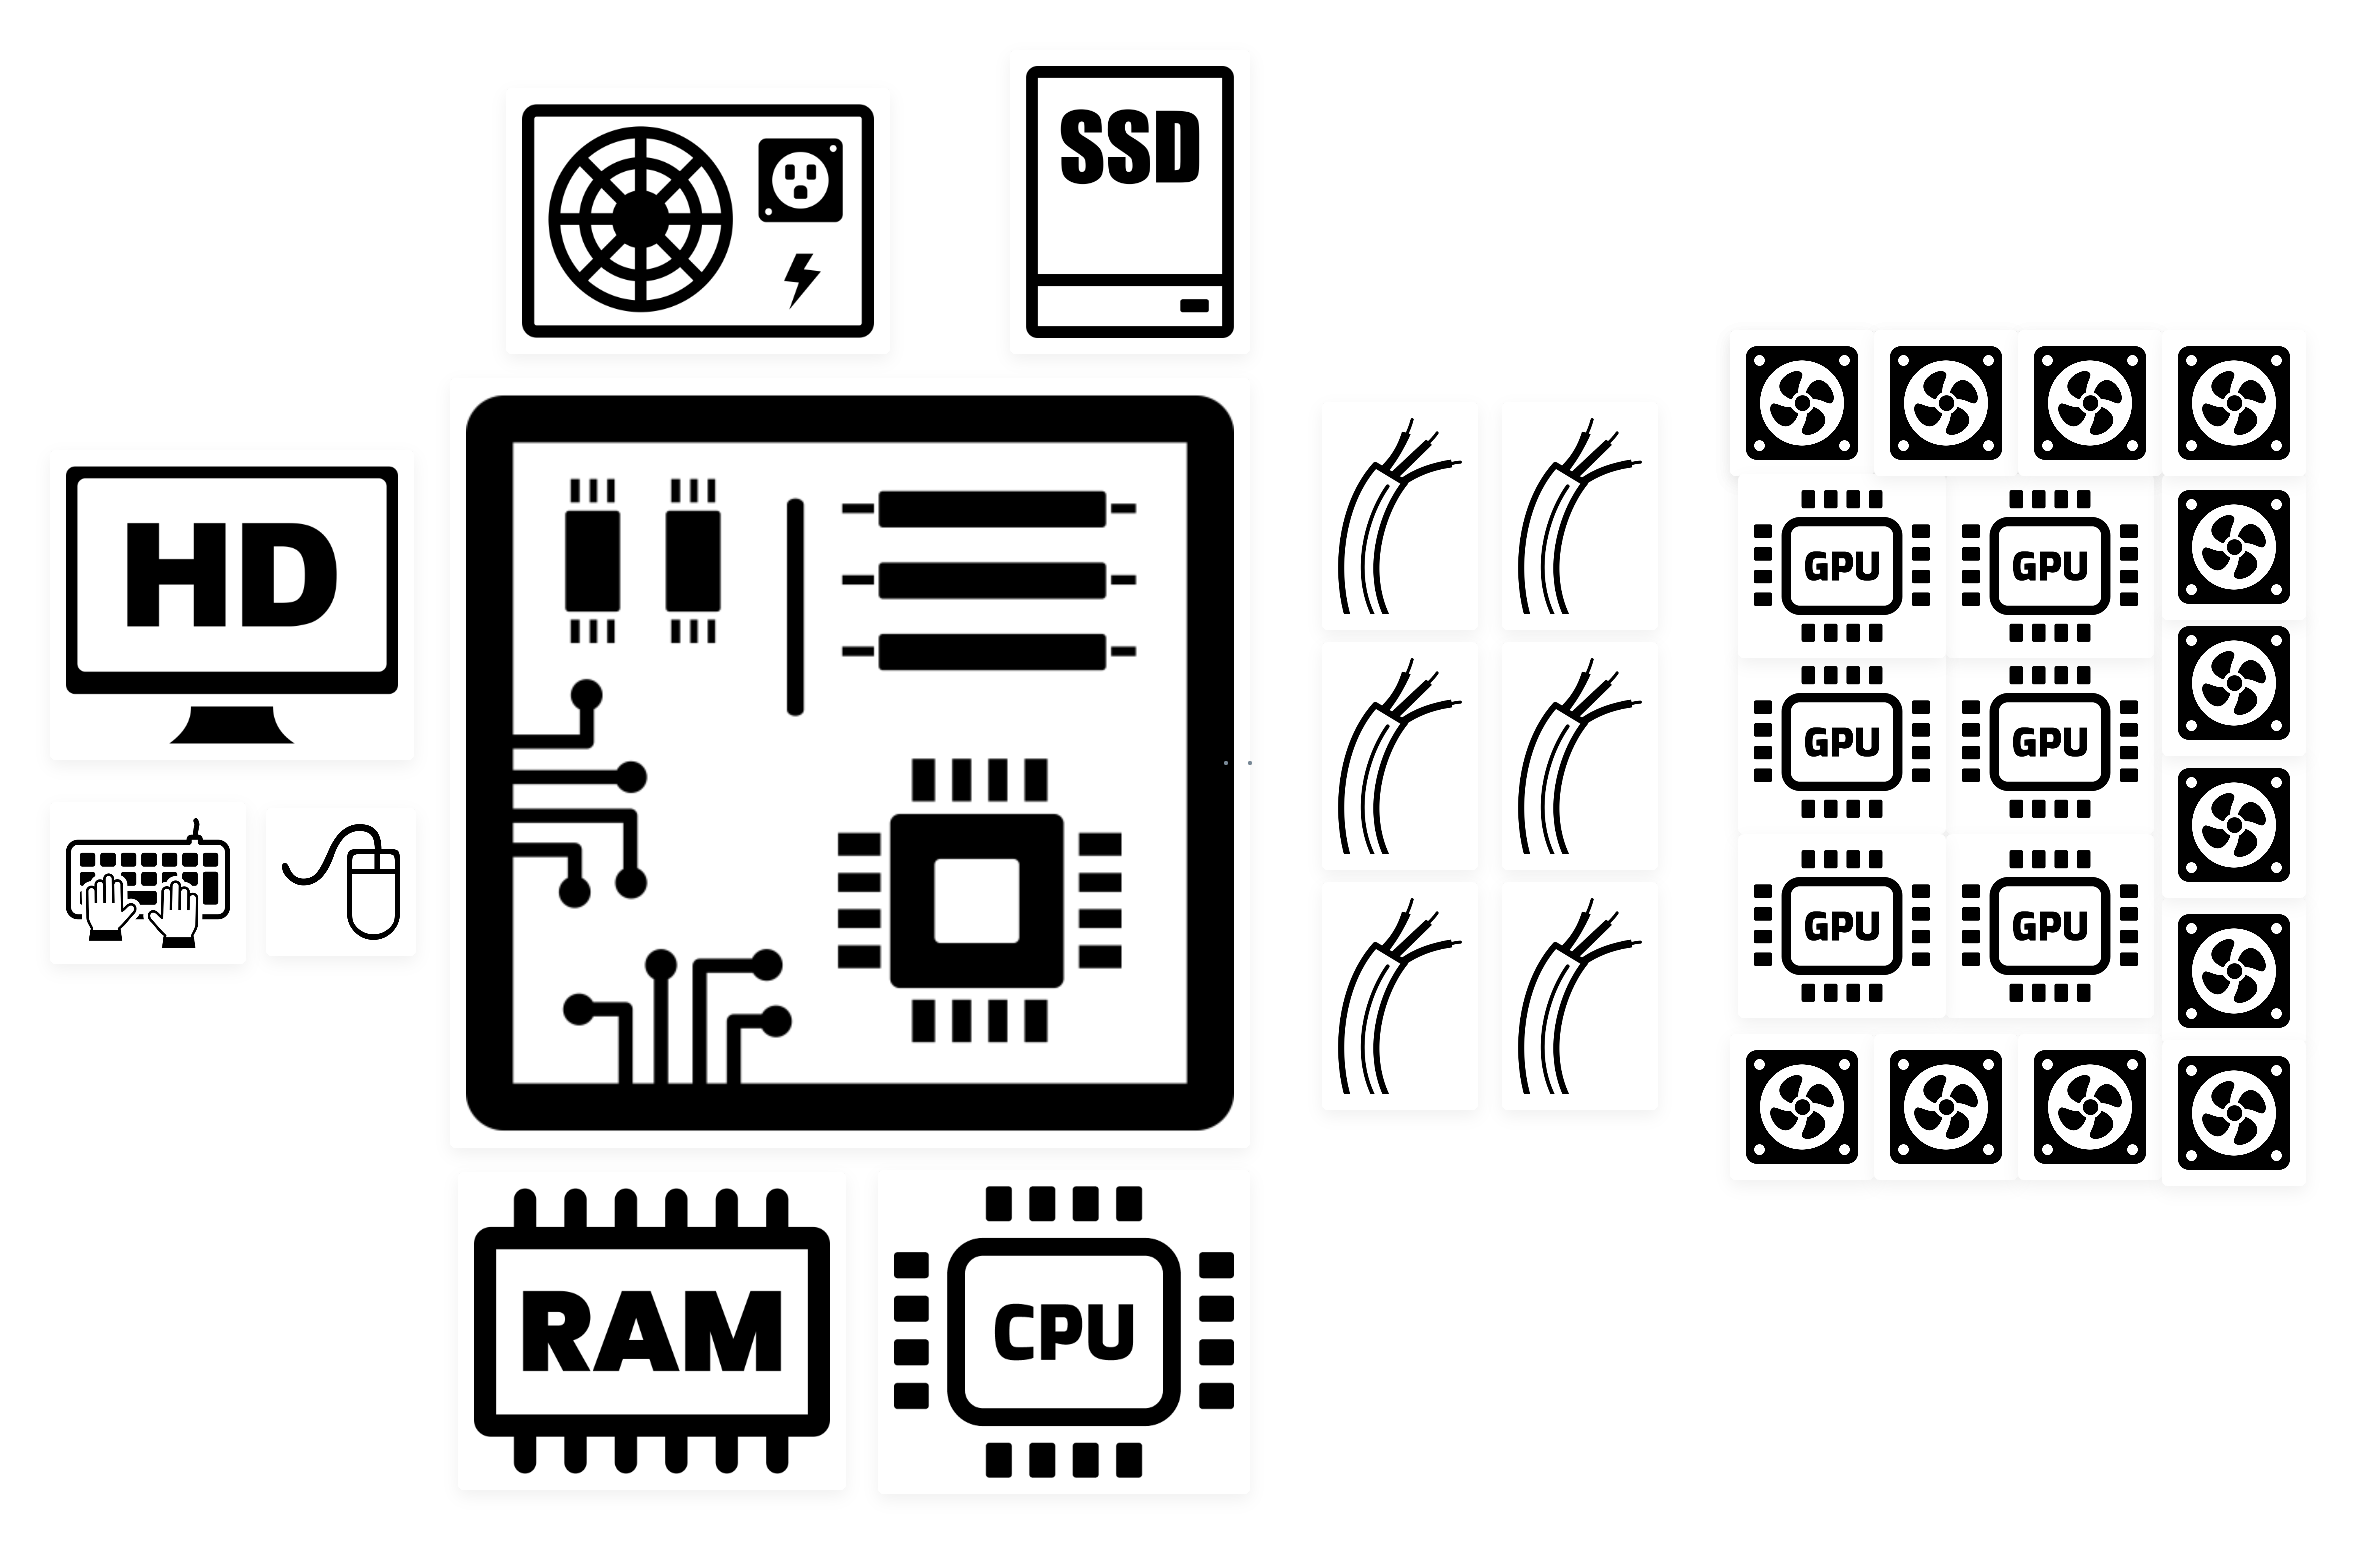
\includegraphics[width=0.7\linewidth]{RIG_ARCH1.png}\\
	\text{Fonte: Desenvolvido pelo autor com assets open-source}
	
\end{figure}   
\subsubsection{Sistemas operacionais} \index{Sistemas Operacionais}
O sistema operacional no qual o aluno faz a pesquisa é indiferente uma vez que as ferramentas de pesquisa a serem utilizadas funcionam de forma igual em todos os sistemas operacionais. Já o sistema operacional que é instalado no equipamento não tem seus custos considerados pois existem excelentes opções open-source que não possuem perdas de desempenho se comparados com seus concorrentes. 

\section{Guia para o professor e guia para o \textit{Hands on!}}\index{Hands On} \label{profguide}

Caro professor, seguem a seguir orientações para uma melhor desenvolvimento desta atividade. Sem perda de generalidade, vamos estipular como objetivo iniciar noso interesse em minerar\index{Mineração} a criptomoeda ETH,\index{Ethereum} que possui grande abrangência de conhecimento na comunidade e possui atualmente a maior lucratividade média de acordo com sua dificuldade de obtenção. Nesta atividade usaremos a calculadora de lucros \textit{Whattomine}\footnote{O professor pode utilizar outras calculadoras disponíveis conforme \ref{opcoes}}, que possuem as práticas mais simplificadas para esta atividade.  Primeiro, inicie navegando para \cite{WTM} \index{Whattomine}. Em seguida, pode-se sugerir que um aluno selecione um modelo de placa de vídeo. Quando uma GPU \textit{Nvidia} for selecionado, o botão se tornará verde, e quando uma GPU \textit{AMD} \index{GPU} for selecionado, o botão se tornará vermelho. Isto auxilia o alunos no momento da pesquisa de preços pois um bom padrão de pesquisa pode ser \textit{" <marca> + <modelo> + preço"}
 
\begin{figure}[H]
	\centering
	\caption{Guia de cores dos botões de seleção de GPUs}
	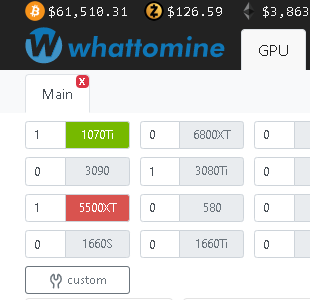
\includegraphics[width=0.5\linewidth]{whattomine_tools1.png}\\
	\text{Fonte: \cite{WTM}}\index{Whattomine}
	
\end{figure}

Para padronização dos procedimentos e simplificação dos cálculos, definimos então somente uma unidade do modelo selecionado e não consideremos inicialmente os custos energéticos. Tais cálculos serão feitos na planilha piloto. Como nosso objetivo é minerar ETH\footnote{Uma forma de variação desta atividade é que cada aluno faça um comparativo das diferentes criptomoedas com um mesmo equipamento}, selecionemos os dados no campo ethash\index{Ethereum} 

\begin{figure}[H]
	\centering
	\caption{Outras opções da calculadoras}\label{opcoes}
	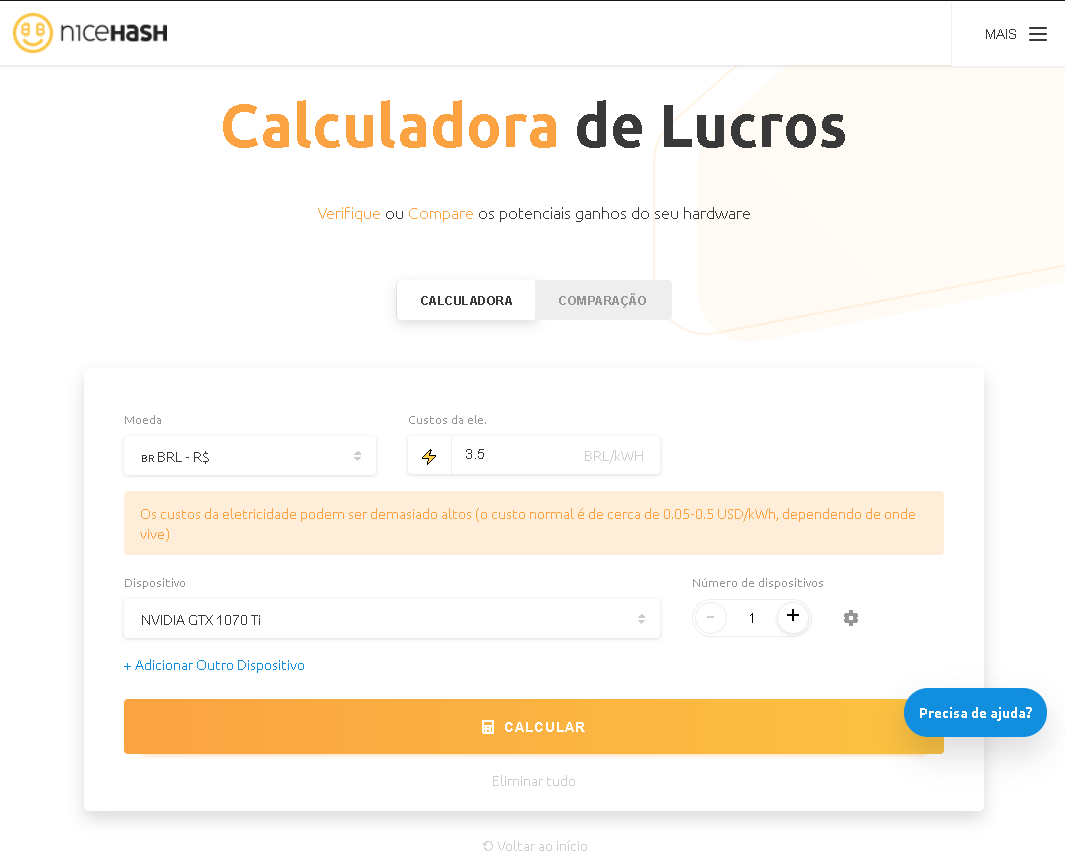
\includegraphics[width=0.4\linewidth]{Nicehash_1.png}
	\includegraphics[width=0.4\linewidth]{minerstat_1.png}\\
	\text{Fonte: \cite{NICE} e \cite{MINER}}
\end{figure}

\begin{figure}[H]\label{algorits}
	\centering \index{Calculadoras}
	\caption{Exemplos de diferentes algorítmos de mineração disponíveis nas calculadoras}
	\subfloat[Nicehash]{\label{a}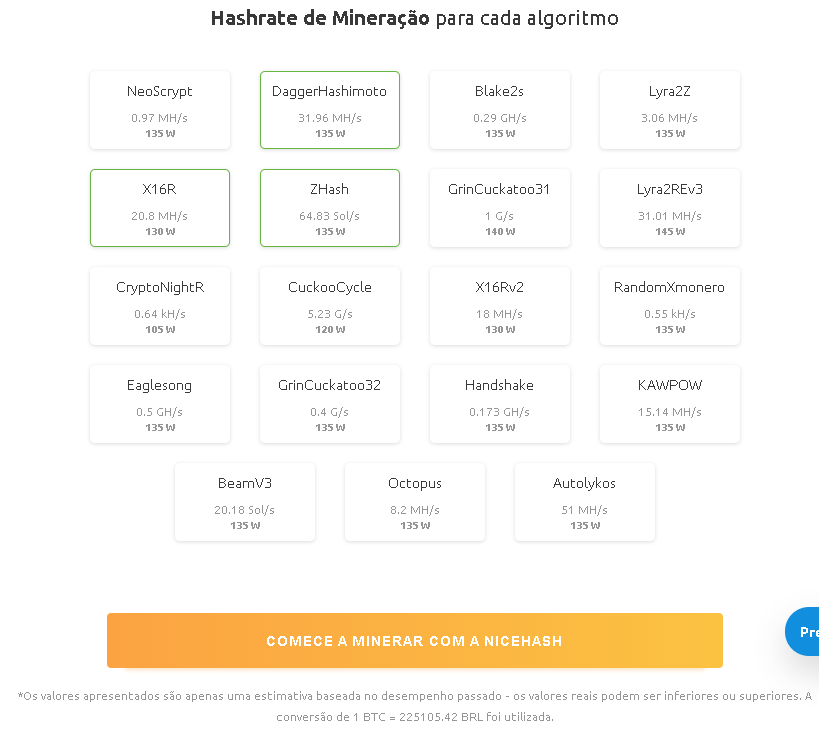
\includegraphics[width=0.5\linewidth]{Nicehash_2.png}}\hfill
	\subfloat[Minerstat]{\label{b}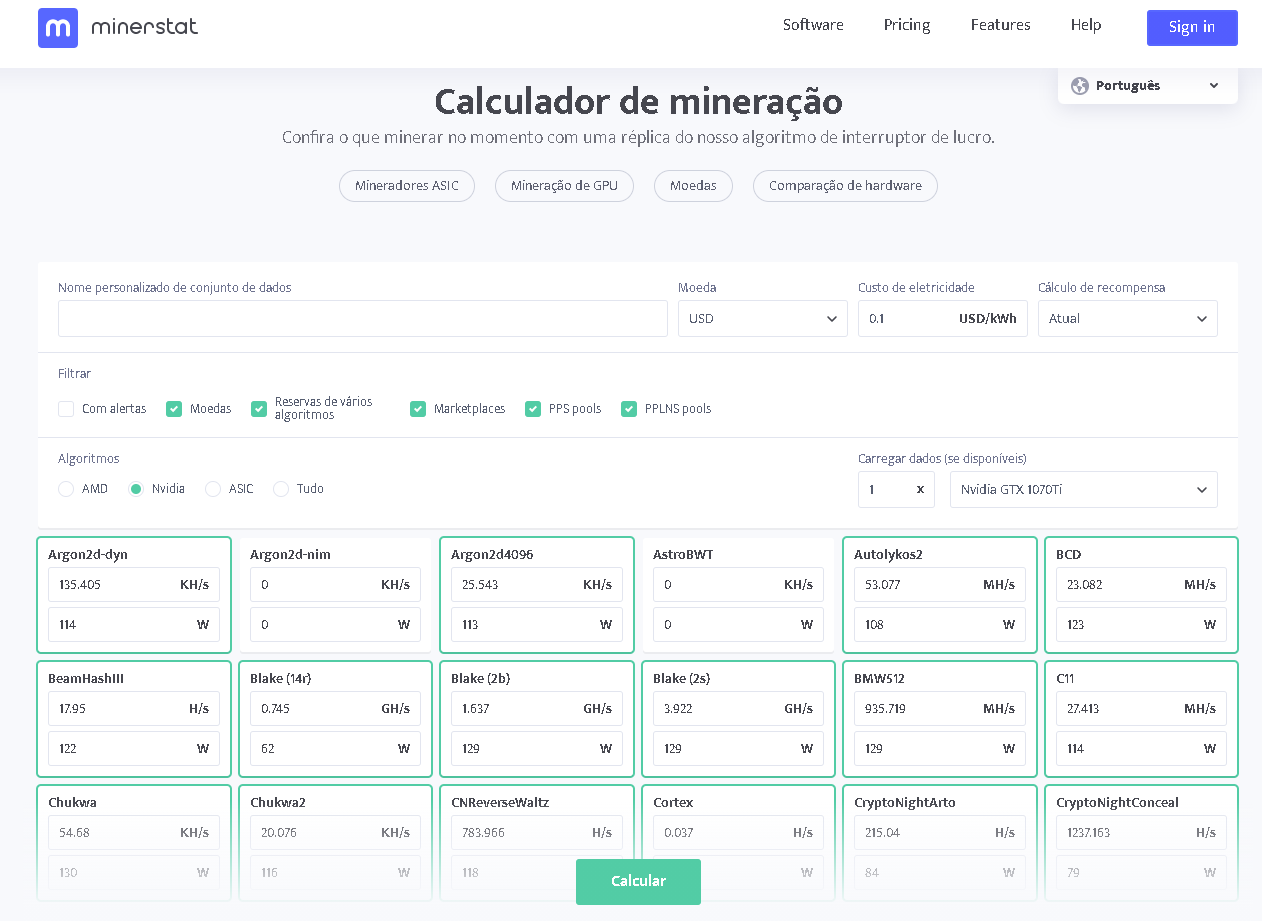
\includegraphics[width=0.48\linewidth]{Minerstat_1.png}}\par 
	\subfloat[Whattomine]{\label{c}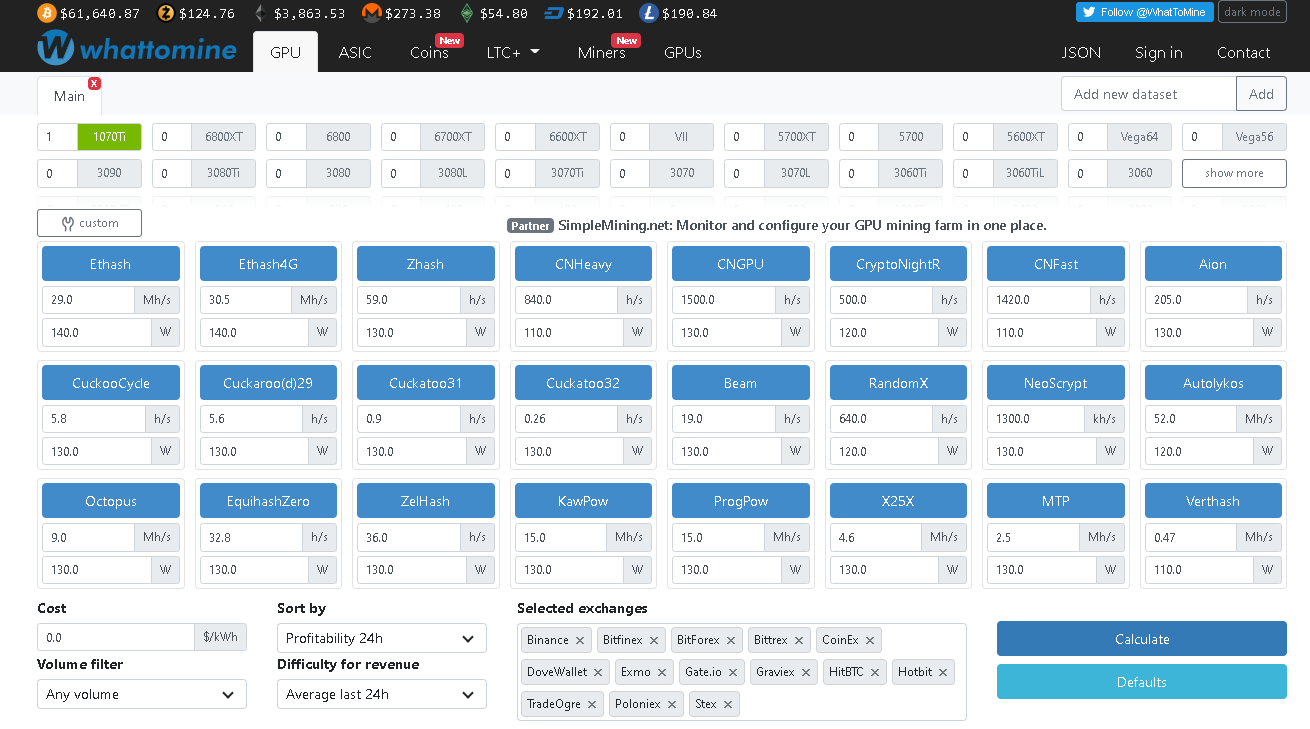
\includegraphics[width=0.48\linewidth]{Whattomine_2.png}}\\
	\text{Fonte: \cite{NICE}, \cite{MINER} e \cite{WTM}} \index{Whattomine}
	\label{fig}
\end{figure}


Conforme a tabela disponível na calculadora logo abaixo das opções, tomemos então nota 
\subsection{Orientações gerais para uso da planilha piloto}
\begin{itemize} \index{Cálculos em planilha}
	\item Para calcular de forma simples o valor do kilowatt/hora no mês específico basta tomar nota o valor total da conta e dividir pelo número de kilowatts gastos no referente mês. Tome nota que existem fatores que podem aumentar ou diminuir este valor para outros meses, sendo este o sistema bandeiras tarifárias, que indicam se haverá ou não acréscimo no valor da energia a ser repassada ao consumidor final, em função das favorabilidade da geração de eletricidade, aumento ou abatimento de impostos municipais, estaduais e federais, entre outros.
	\item O consumo energético mensal é calculado da seguinte forma:
	Toma-se o consumo em kW de uma GPU,\index{GPU} \index{RIG} multiplica-se pelo número de GPUs na RIG, e deste valor soma-se o fator de consumo do RIG que nada mais é que o consumo esperado dos outros componentes do RIG fora as GPUs. Este valor tem base empírica.   
	\item \index{Câmbio} A cotação de USD para BRL acontece de forma automática pelo serviço gerenciado da google. Por isso, há um aviso de exoneração abaixo afirmando que "As cotações não são provenientes de todos os mercados e podem ter um atraso de até 20 minutos. As informações são fornecidas "no estado em que se encontram" e apenas para fins informativos, não para fins comerciais ou consultoria". 
	\begin{equation}\label{key1}
		=GOOGLEFINANCE("Currency:USDBRL";"Average")
	\end{equation}
	\item A planilha foi projetada para que, caso o professor opte em usá-la em aula, que os alunos devam alterar somente os campos em cor verde.
	\item Para realizar um cálculo preciso do consumo do RIG, \index{RIG} obtendo assim o consumo energético mensal, foi utilizada a seguinte fórmula: 
	\begin{equation}\label{key}
		= (B9*B12+\$M\$11)*\$L\$21*\$L\$11
	\end{equation} 
	Sendo assim, caso a planilha não seja usada pelos alunos, pode-se recomendar a pesquisa da taxa de câmbio no momento da aula, daí basta multiplicar a valor encontrado pela calcula pela taxa encontrada.
	\item \index{Marketplace} Para a pesquisa em marketplaces, recomendam-se lojas de varejo já conhecidas pelas comunidades de tecnologia. Bons exemplos são como kabum.com, terabyteshop.com e aliexpress.com \footnote{Por se tratar de uma loja internacional, para esta entrada em específico pode-se incentivar os alunos a considerarem uma chance de taxação, sendo 60\% do valor declarado do produto como imposto devido a fiscalização da Receita Federal Brasileira (RFB). Leia mais sobre isto em \cite{PROMOBIT}} e entre outros.
\end{itemize}





  
 

\section{Exemplo de plano de aula} \index{Plano de Aula}


\begin{table}[H]
	\centering
\begin{tabular}{|l|r|}
	\hline
	\multicolumn{2}{|l|}{} \\
	\multicolumn{2}{|l|}{Colégio Estadual Minerador Satoshi Nakamoto} \\
	\multicolumn{2}{|l|}{} \\
	\hline
	\multicolumn{2}{|l|}{} \\
	\multicolumn{2}{|l|}{Projeto de intervenção com \textit{hands-on}: Mineração, vale a pena investir?} \\
	\multicolumn{2}{|l|}{} \\
	\hline
	& \\
	Disciplina & Matemática \\
	& \\
	\hline
	& \\
	Turma & 902 \\
	& \\
	\hline
	& \\
	Alunos & 21 \\
	& \\
	\hline
	& \\
	Ano & 9\textdegree ano \\
	& \\
	\hline
	& \\
	Tempo de aula & 100 minutos \\
	& \\
	\hline
	& \\
	Tema da atividade & \multirow{3}{11cm}{Nesta atividade vamos estudar o tempo de recuperação de investimentos em um RIG \index{RIG} de mineração, tomando como base os cálculos realizados em uma calculadora de lucros.} \\	
	& \\	
	& \\	
	& \\	
	\hline
	& \\
	Objetivo & \multirow{4}{11cm}{Perfilhar novas concepções na matemática financeira, exibindo e simulando uma situação por meio de pesquisa temática. Instar a compreensão da  matemática dentro do escopo proposto, tornando significativo sua aplicação e desenvolvimento.}  \\
	& \\
	& \\	
	& \\	
	& \\
	& \\
	\hline
	& \\ 
	Conteúdo & \multirow{3}{11cm}{Para os alunos nenhum conteúdo fora do escopo escolar é mandatório para esta atividade, necessitando somente do acompanhamento das atividades previamente realizadas em sala de aula. Recomenda-se que o professor já tenha ministrado aulas anteriores com escopo de finanças.} \\
	& \\
	& \\
	& \\	
	& \\	
	& \\
	\hline
	& \\
	Referências &  \multirow{1}{11cm}{BNCC.EF09MA18, BNCC.EF08MA04, BNCC.EF05MA19, }\\
& \\
	\hline
\end{tabular}
		\caption{Exemplo de plano de aula}
\end{table}

\subsection{Materiais necessários e opicionais}
\begin{itemize}
	\item Acesso a internet (obrigatório)
	\item Acesso a hardware com acesso a internet (obrigatório) 
	\item Acesso a softwares para ferramentas de pesquisa (obrigatório)
	\item Acesso ao demonstrativo de gastos na energia elétrica da residência do aluno (obrigatório)
	\item Disponibilidade de software de edição de planilhas como o \textit{Microsoft Excel}, \textit{Google Sheets} ou \textit{Libreoffice Calc} (opcional) 
	
\end{itemize}





\subsection{Metodologia} \index{Metodologia}
\begin{enumerate}
	\item Reservar com a coordenação da escola ou departamento apropriado um horário no laboratório de informática. 
	
	Nota importante: É de todo oportuno trazer à baila que, constatando a impossibilidade de comparecimento ao espaço de do laboratório, outrora por mau funcionamento do equipamento fornecido ou impedimento independente, recomenda-se que o docente aplicador tenha equipamento próprio como um projetor. Outrossim, adaptando a metodologia, manter os alunos em sala de aula, e seguir dali conforme metodologia, apresentando em slides a exibição dos dados e websites aqui propostos. A fim de corroborar com o prevalecimento da ordem pública, fica vetado em primeira mão para objeto de desvio de atenção o uso de celulares ,além do uso de redes sociais.
	
	\item No dia e horários reservados, o professor deve entrar em sala, realizar a presença dos alunos, transmitir informações e avisos necessários. Em seguida, antes de acessar os equipamentos, coletar os demonstrativos de gastos na energia elétrica da residência dos alunos \footnote{Se os alunos forem todos do mesmo município, supondo uma aula presencial, apenas um dos demonstrativos é suficiente}, em seguida calcular com os alunos a valor cobrado do kilowatt pela companhia energética\footnote{Veja mais na seção guia do professor em \ref{profguide}}. Orientar os alunos na utilização da planilha fornecida, ou incentivá-los a construir algo semelhante a planilha piloto\footnote{Conforme também supracitado no guia do professor, há um link para download da planilha piloto no apêndice deste documento. (\ref{sheetdownload})} de cálculo de retorno de investimentos por meio da aplicação de edição de planilhas. 
	
	\item Em seguida, orientá-los a acessarem seus navegadores e direcioná-los para a ferramenta de pesquisa favorita. Seguir a atividade incitando a pesquisa de modelos de \index{GPU} GPUs, pesquisarem em Marketplaces os valores médios de compra destes componentes e em seguir utilizar a calculadora de lucros para obter o rendimento de uma GPU por dia, além de seu consumo energético.\index{Marketplace}
	No exemplo, podemos ver as variações nas mais diversas moedas como ETH, RVN, FIRO \index{FIRO} \index{Ravencoin} e muitas outras. Como queremos
	
	\begin{figure}[H]
		\centering
		\caption{Lista de lucratividade média diária de criptomoedas}
		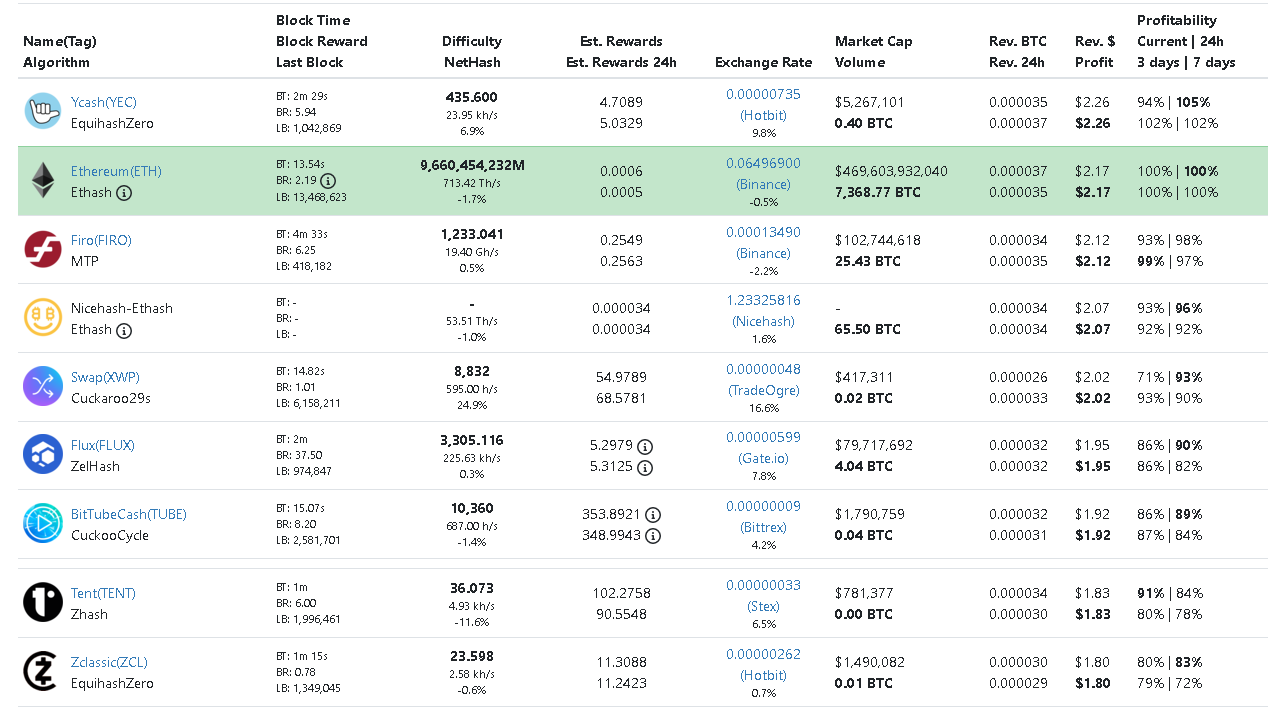
\includegraphics[width=\linewidth]{Whattomine_3.png}
		\text{Fonte: \cite{WTM}}\\ \index{Whattomine}
	\end{figure}
	
	\item Em seguida, deve-se calcular a conversão de câmbio entre BRL e USD, e consequentemente multiplicar tais valores para uma base de cálculo mensal. Daqui subtrai-se o consumo energético e pode-se ter uma ideia de quantos meses são necessários para que os lucros obtidos integralizem o investimento feito inicialmente. 

\end{enumerate}

 \subsection{Avaliação} \index{Avaliação}
 Ao fim da aula, deve ser observado se os alunos tiveram as capacidades de acompanhar as atividades propostas corretamente, além da participação, e trabalho em grupo. Relevar se surgirem problemas ao tempo de aula, ou se os materiais se tornarem escassos (falhas de \textit{hardware}, interrupções por queda de energia, fenômenos da natureza)
 
 \section{Exemplo de resultado}
 \begin{figure}[H] \label{result1}
 	\centering
 	\caption{Planilha de cálculo de lucros, parte 1}
 	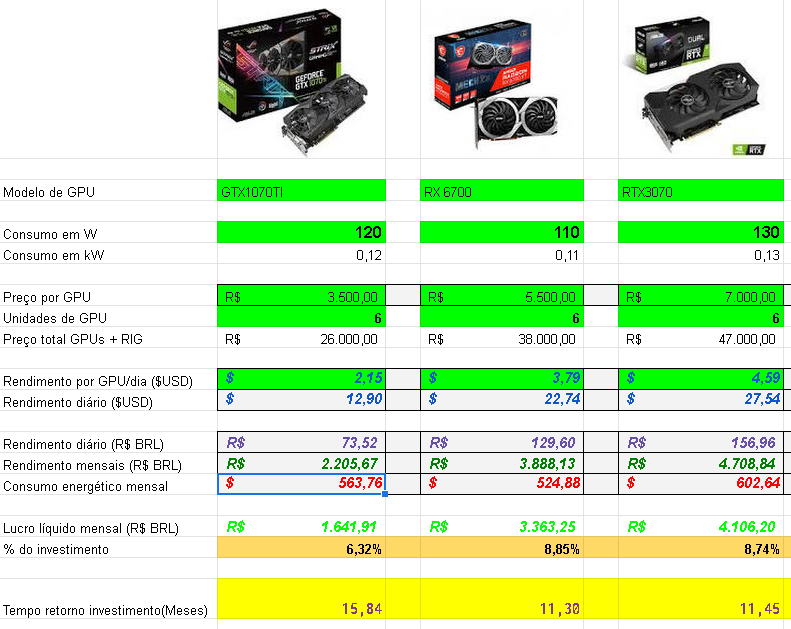
\includegraphics[width=0.8\linewidth]{planilha_1.png}
 	\text{Fonte: Desenvolvido pelo autor com software de manipulação de planilhas}
 \end{figure}
 
 \begin{figure}[H]\index{Cálculos em planilha}  \label{result2} \label{example_sheet}
 	\centering
 	\caption{Planilha de cálculo de lucros, parte 2}
 	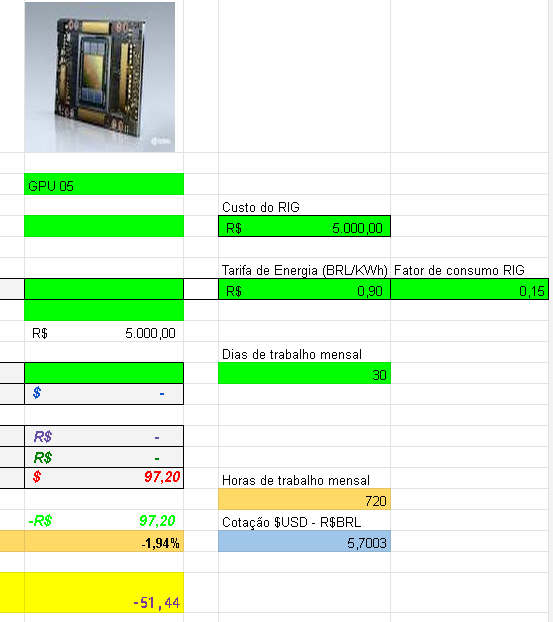
\includegraphics[width=0.5\linewidth]{planilha_2.png}\\
 	\text{Fonte: Desenvolvido pelo autor com software de manipulação de planilhas}
 \end{figure}

 Nas figuras acima, usando a planilha piloto foram realizadas três simulações com parâmetros com GPUs existentes no banco de modelos  em \cite{WTM}, com uma taxa de energia aferida de uma conta de gasto energético real.  Após os cálculos obtiveram-se, respectivamente, 15,84 , 11,30 e 11,45 meses para o retorno de um investimento. Retornando ao questionamento feito em \ref{motiv}, um motorista conseguiria liquidar todo seu investimento neste tempo encontrado? Fica para o leitor responder a esta pergunta.
 






